\subsection{The Thomson Scattering Diagnostic}

The Thomson Scattering (TS) diagnostic is a laser-based optical diagnostic which operates via the eponymous Thomson scattering process. On MST, it is setup to provide $T_e$ measurement, though the physics of the Thomson scattering process is in theory able to provide both temperature and density information about either electrons or ions. Thomson scattering itself can be understood as the limit of Compton scattering of photons on free charged particles at the limit of low photon energy, in this case, free electrons in the plasma. In short, the free electron will scatter incident photons to a new direction while preserving frequency. But individual electrons travels at various speeds and directions and will thus encounter variously blue and red shifted incident photons from the laser, causing the scattered output to experience line broadening analogous to Doppler broadening. In particular, the TS diagnostic takes advantage of incoherence (or non-collective) Thomson scattering in the plasma.  In this case, the wavelength of the incident photons are much smaller than the Debye length of the plasma, thus the plasma will not respond collectively to the light, but instead electrons respond approximately individually. The mechanics of Thomson scattering is best explained in the classical wave-based picture. The incident E-M wave accelerates free electrons in a oscillatory fashion, and as an oscillating charge, the electron radiates E-M waves in all directions with the same frequency with an intensity pattern that varies with the incident angle. In a plasma context, a powerful laser is used to provide the incident light at a specific frequency, and the scattered light is observed. However, the scattered light from a plasma is not the work of a particular electron, but made up from many individual scattering events off of many electrons. The electrons have a distribution of velocities in the direction of the incident beam, and as mentioned above, scatters the incident beam over a distribution of wavelengths. Thus, the intensity of the scattered light from a plasma is a function of scattering angle, electron density, as well as electron temperature. This intensity function is further modified due to relativistic effects important for hot plasmas ($>1$ keV). 
 
The spectral intensity $S(\epsilon, \theta, \alpha)$ (the directed scattered power per solid angle per normalized  wavelength shift $\epsilon$) due to scattering by a Maxwellian distribution of electrons are first calculated by Zhuravlev and Petrov\cite{Zhuravlev1979} and expanded upon by Seldon\cite{Seldon1980} for routine analysis as follows:
\begin{align}
    S(\epsilon, \theta, \alpha) &= \frac{c(\alpha)}{A(\epsilon, \theta)}e^{-2\alpha B(\epsilon,\theta)} \label{eq:Sheldon}\\
    &\text{where:}\nonumber\\
    A (\epsilon, \theta) &= (1+\epsilon)^2\sqrt{1(1- \cos\theta)(1+\epsilon) + \epsilon^2} \nonumber\\
    B (\epsilon, \theta) &= \sqrt{1 + \frac{\epsilon^2}{2(1-\cos\theta)(1+\epsilon)}} - 1 \nonumber\\
    c (\alpha) &= \sqrt{\frac{\alpha}{\pi}}(1 - \frac{15}{16}\alpha^{-1} + \frac{345}{512}\alpha^{-2} + \ldots) &\text{for } \alpha \gg 1 \nonumber
\end{align}
and $\alpha \equiv \frac{1}{2}\frac{m_ec^2}{kT_e}$, $\epsilon = \frac{\lambda_s}{\lambda_i}$ is the normalized wavelength shift, and $\theta$ is the scatter angle. This analytical calculation does not account for depolarization effects, but observations have shown that for the characteristic parameters of MST, the depolarization effects can be safely ignored\cite{Seldon1982}. 

\begin{figure}[!htb]
	\centering
	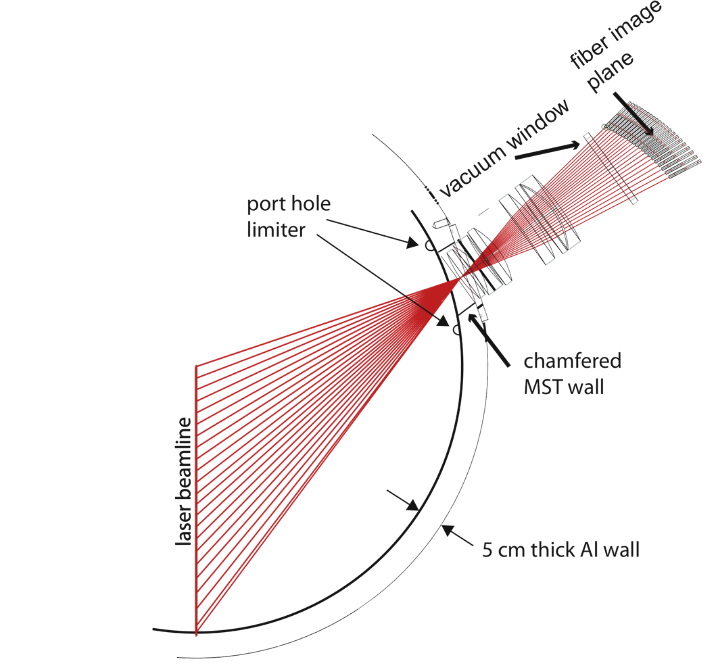
\includegraphics[width = 0.9\linewidth]{./implementation/diagnostics/ts_optics_diagram.png}
	\label{fig:ts_optics_diagram}
	\caption[Diagram of Thomson scattering optics and sight lines]{Diagram of Thomson scattering optics and sight lines. The scattering angle in equation \ref{eq:Sheldon} are dictated by angle made by the red view paths and the laser beam line. (Reproduced from J. Reusch.\cite{Reusch2011})}
\end{figure}

In MST, the TS diagnostic has 21 sight-lines. The scattering angle for a particular sight-line is fixed by the geometry of the viewing optics and ranges from $\sim 108\degree$ to $\sim 143\degree$. The wavelength dependence is observed via an array of polychromators equipped with avalanche photo-diodes digitized at 100MHz to help separate the scattered laser light from the background (digitized both before and after the laser pulse). The temperature $T_e$ is found via least \chisq\ fitting of these observations. The temperature measurements are localized by the intersection of the laser beam path and the viewing geometry, allowing direct $T_e$ profile measurements without relying on inversion techniques. The main limiting factor of TS diagnostics are the fact very little of the incident beam power is scattered (ie. the cross section is very small), and thus it relies on a very powerful pulsed laser (pulse energies $\sim$ Joule) to provide the incident beam. Such lasers are often limited in their repetition rate due to the technical difficulties with heat in the lasing medium, thereby limiting the ability to diagnose fast phenomenon. MST's TS system is powered by two laser ``backends.'' The older ``work-horse'' system is based on a pair of off-the-shelf Q-switching Nd:YAG lasers operating at 1064nm. A series of upgrades have been made to the Pockel cell drivers (that are responsible for Q-switching) and power supplies that significantly increase the repetition rate achieved to up to $\sim 1$~kHz per laser over $\sim 15$~ms of active time\cite{DenHartog2010}. In standard operation, the two lasers' timing are staggered in such a way to achieve effectively a 2~kHz pulse rate. This is the mode used to take the data related to this research, as it focuses more on the slower time scale effects the electron $T_e$ have on the ions. The effective TS frequency of 2~kHz affects the rate at which the plasma kinetic profiles are updated and sets the evolution timescale of the model. This issue will be addressed in more detail in section \ref{sec:time_blocks_and_steps}. For studies of faster plasma phenomenon, the Spectron lasers can also be operated in a pulse-burst mode\cite{DenHartog2010} where bursts very fast pulses are produced and repeated. A typical repetition rate in this mode produces 8 pulses at 25~kHz, and these bursts themselves repeats at 1~kHz. The TS system also has an alternative custom-built laser system commonly called the Fast Thomson system despite the fact that the `regular' TS system is already very fast. The Fast Thomson system can be operated at a repetition rate of up to 333~kHz for 3-4 pulses, or 100~kHz for 44 pulses\cite{Young2015}, giving it exceptional capabilities to resolve fast $T_e$ dynamics. It is, however, not relevant this this work. 

A detailed overview of MST's TS system can be found in the thesis of J. Reusch\cite{Reusch2011}, and an recent comprehensive treatment of TS theory is available by Prunty\cite{Prunty2014}.
